\documentclass[aspectratio=169,10pt]{beamer}

\usepackage[utf8]{inputenc}
\usepackage[T1]{fontenc}
\usepackage[english]{babel}
\usepackage{amsmath,amssymb,mathtools}
\usepackage{booktabs}
\usepackage{listings}
\usepackage{tikz}
\usetikzlibrary{arrows.meta,calc,positioning}

% ---------- visual system ----------
\definecolor{Ink}{HTML}{14213D}
\definecolor{Navy}{HTML}{173B57}
\definecolor{Teal}{HTML}{167D7F}
\definecolor{Mint}{HTML}{DCEFED}
\definecolor{Gold}{HTML}{D9A441}
\definecolor{Sand}{HTML}{F6F0E5}
\definecolor{Red}{HTML}{B74343}
\definecolor{SoftRed}{HTML}{F7E4E2}
\definecolor{Slate}{HTML}{5B6870}
\definecolor{Mist}{HTML}{EEF3F5}
\definecolor{CodeBg}{HTML}{F4F6F8}

\usetheme{default}
\usefonttheme{professionalfonts}
\setbeamertemplate{navigation symbols}{}
\setbeamersize{text margin left=0.62cm,text margin right=0.62cm}
\setbeamercolor{normal text}{fg=Ink,bg=white}
\setbeamercolor{structure}{fg=Teal}
\setbeamercolor{frametitle}{fg=white,bg=Navy}
\setbeamerfont{frametitle}{size=\large,series=\bfseries}
\setbeamerfont{title}{size=\LARGE,series=\bfseries}
\setbeamerfont{subtitle}{size=\normalsize}
\setbeamercolor{block title}{fg=white,bg=Navy}
\setbeamercolor{block body}{fg=Ink,bg=Mist}
\setbeamercolor{block title alerted}{fg=white,bg=Red}
\setbeamercolor{block body alerted}{fg=Ink,bg=SoftRed}
\setbeamercolor{block title example}{fg=white,bg=Teal}
\setbeamercolor{block body example}{fg=Ink,bg=Mint}

\setbeamertemplate{frametitle}{%
  \nointerlineskip
  \begin{beamercolorbox}[wd=\paperwidth,ht=0.74cm,dp=0.20cm,leftskip=0.62cm]{frametitle}
    \usebeamerfont{frametitle}\insertframetitle
  \end{beamercolorbox}
}

\setbeamertemplate{footline}{%
  \leavevmode
  \hbox{%
    \begin{beamercolorbox}[wd=.82\paperwidth,ht=2.55ex,dp=1.05ex,leftskip=.62cm]{author in head/foot}%
      \color{Slate}\scriptsize AI and Economic Modeling \hspace{0.7em}\textcolor{Teal}{\rule{0.8em}{0.12em}}\hspace{0.7em} Quispe--Xu (2026)
    \end{beamercolorbox}%
    \begin{beamercolorbox}[wd=.18\paperwidth,ht=2.55ex,dp=1.05ex,rightskip=.62cm plus1fil]{date in head/foot}%
      \hfill\color{Slate}\scriptsize\insertframenumber/\inserttotalframenumber
    \end{beamercolorbox}%
  }
}

\newcommand{\strong}[1]{\textcolor{Teal}{\textbf{#1}}}
\newcommand{\weak}[1]{\textcolor{Gold}{\textbf{#1}}}
\newcommand{\warning}[1]{\textcolor{Red}{\textbf{#1}}}
\newcommand{\source}[1]{\textcolor{Slate}{\scriptsize #1}}

\newcommand{\metric}[3]{%
  \begin{beamercolorbox}[wd=\linewidth,sep=0.11cm,center,rounded=true]{block body example}
    {\color{Teal}\Large\bfseries #1}\par
    {\scriptsize #2}\par
    {\tiny\color{Slate}#3}
  \end{beamercolorbox}%
}

% ---------- Lean source rendering ----------
\lstdefinelanguage{Lean}{
  morekeywords={theorem,def,by,have,exact,if,then,else,with,fun,intro,apply,let,letI,show},
  sensitive=true,
  morecomment=[l]{--},
  morestring=[b]"
}
\lstset{
  language=Lean,
  basicstyle=\ttfamily\fontsize{6.0}{6.8}\selectfont,
  keywordstyle=\color{Navy}\bfseries,
  commentstyle=\color{Slate}\itshape,
  backgroundcolor=\color{CodeBg},
  frame=single,
  rulecolor=\color{Mist},
  framesep=3pt,
  xleftmargin=2pt,
  xrightmargin=2pt,
  columns=fullflexible,
  keepspaces=true,
  showstringspaces=false,
  breaklines=true,
  literate=
    {ℝ}{{$\mathbb{R}$}}1
    {ℤ}{{$\mathbb{Z}$}}1
    {ℕ}{{$\mathbb{N}$}}1
    {≤}{{$\leq$}}1
    {∧}{{$\wedge$}}1
    {¬}{{$\neg$}}1
    {∀}{{$\forall$}}1
    {∈}{{$\in$}}1
    {∃}{{$\exists$}}1
    {→}{{$\to$}}1
    {·}{{\textcolor{Teal}{\textbullet}}}1
}

\title{Agentic Delegation and the Language Frontier of Software Developers}
\subtitle{A model, GitHub evidence, and what formal verification changes}
\author{Carlos G\'omez Puican}
\date{September 2026}

\begin{document}

% -------------------------------------------------------------------
\begin{frame}[plain]
  \begin{tikzpicture}[remember picture,overlay]
    \fill[Navy] (current page.north west) rectangle ([yshift=-1.20cm]current page.north east);
    \fill[Teal] (current page.south west) rectangle ([yshift=0.16cm]current page.south east);
    \fill[Mint] ([xshift=10.7cm,yshift=-1.20cm]current page.north west)
      -- (current page.north east) -- ([yshift=-4.0cm]current page.north east) -- cycle;
  \end{tikzpicture}

  \vspace{0.72cm}
  {\color{Teal}\small\bfseries AI AND ECONOMIC MODELING \hspace{0.6em}\textcolor{Gold}{/}\hspace{0.6em} REPOSITORY 3}

  \vspace{0.48cm}
  {\color{Ink}\fontsize{22}{25}\selectfont\bfseries
    Agentic Delegation and the\\[-0.05cm]
    Language Frontier of Software Developers\par}

  \vspace{0.18cm}
  {\color{Slate}\large A model, GitHub evidence, and what formal verification changes\par}

  \vspace{0.46cm}
  \begin{beamercolorbox}[wd=0.83\textwidth,sep=0.20cm,rounded=true]{block body example}
    \textbf{Research question.} Does agentic AI only raise productivity in languages a developer already uses, or can delegation make previously infeasible languages economical to enter?
  \end{beamercolorbox}

  \vfill
  {\small Carlos G\'omez Puican \hspace{0.5em}\textcolor{Gold}{\textbullet}\hspace{0.5em} September 2026}\par
  \vspace{0.15cm}
  {\footnotesize\color{Slate}Alexander Quispe \& Kevin Xu (2026), \emph{Agentic Delegation and the Language Frontier of Software Developers: A Model and Evidence from Claude Code on GitHub}. arXiv:2605.25438v2.}
  \vspace{0.26cm}
\end{frame}

% -------------------------------------------------------------------
\begin{frame}{1. The mechanism: skill frontier $\neq$ production frontier}
  \vspace{-0.08cm}
  \begin{columns}[T,onlytextwidth]
    \begin{column}{0.47\textwidth}
      \begin{block}{Unaided human-skill frontier}
        Languages in which the developer can personally execute with language-specific skill $s_{ik,t}$.

        \medskip
        It is sticky because language-specific capital is costly to acquire and uncertain in a new language.
      \end{block}
    \end{column}
    \begin{column}{0.47\textwidth}
      \begin{exampleblock}{Production frontier}
        Languages in which the developer can \emph{profitably deliver} using any mode currently in the production menu.

        \medskip
        Delegated code can belong to this frontier without implying unaided mastery.
      \end{exampleblock}
    \end{column}
  \end{columns}

  \vspace{0.20cm}
  \[
    V^{g}_{ik,t}=\max_{m\in\mathcal M_g}V^m_{ik,t},
    \qquad
    Z^{g}_{ik,t}=\mathbf 1\!\left[V^{g}_{ik,t}\ge 0\right],
    \qquad
    N^g_{it}=\sum_k Z^g_{ik,t}.
  \]

  \begin{center}
    \strong{Economic object:} an extensive participation margin, not a claim that the human suddenly learns every activated language.
  \end{center}
\end{frame}

% -------------------------------------------------------------------
\begin{frame}{2. One opportunity, three production modes}
  \vspace{0.05cm}
  \begin{columns}[T,onlytextwidth]
    \begin{column}{0.31\textwidth}
      \begin{block}{S \; Solo}
        The developer executes.
        \[
          V^S=\omega+s\mu-\frac{\rho s^2}{2\pi}-b
        \]
        \scriptsize Expected human output is offset by activation cost and risk from the uncertain developer--language match.
      \end{block}
    \end{column}
    \begin{column}{0.31\textwidth}
      \begin{block}{C \; Conversational AI}
        The developer still executes.
        \[
          V^C=V^S+\gamma s-r_C
        \]
        \scriptsize Assistance is proportional to existing language-specific skill: useful advice must still be read, adapted, and run.
      \end{block}
    \end{column}
    \begin{column}{0.31\textwidth}
      \begin{exampleblock}{D \; Delegation}
        The agent executes share $\lambda$.
        \[
          (1-\lambda)s\mu
          \quad+\quad
          \lambda a z(A)
        \]
        \scriptsize Human execution is partly replaced by agent execution under human specification and verification.
      \end{exampleblock}
    \end{column}
  \end{columns}

  \vspace{0.18cm}
  \begin{center}
    \weak{The comparison is not ``no AI'' versus ``AI''.}
    It is $\mathcal M_1=\{S,C\}$ versus $\mathcal M_2=\{S,C,D\}$.
  \end{center}
\end{frame}

% -------------------------------------------------------------------
\begin{frame}{3. Solo and conversational entry: augmentation needs a foothold}
  \begin{columns}[T,onlytextwidth]
    \begin{column}{0.54\textwidth}
      \begin{align*}
        \omega\ge T^S
        &\equiv b-s\mu+\frac{\rho s^2}{2\pi},\\[0.15cm]
        T^C
        &=T^S-(\gamma s-r_C),\\[0.15cm]
        T^1
        &=\min\{T^S,T^C\}
          =T^S-\max\{0,\gamma s-r_C\}.
      \end{align*}
    \end{column}
    \begin{column}{0.42\textwidth}
      \begin{alertblock}{Paper Assumption 1}
        For unfamiliar languages with skill $\underline{s}$,
        \[
          \gamma\underline{s}-r_C\le 0.
        \]
        For familiar languages with skill $\bar{s}$,
        \[
          \gamma\bar{s}-r_C>0.
        \]
      \end{alertblock}
    \end{column}
  \end{columns}

  \vspace{0.16cm}
  \begin{beamercolorbox}[wd=\textwidth,sep=0.19cm,rounded=true]{block body example}
    \centering
    \textbf{Unfamiliar language:}\quad
    $\gamma\underline{s}-r_C\le 0\ \Longrightarrow\ T^1=T^S$.\quad
    Conversational AI does not move this entry margin \emph{under the maintained assumption}.
  \end{beamercolorbox}
\end{frame}

% -------------------------------------------------------------------
\begin{frame}{4. Delegated surplus and the new threshold}
  \small
  \begin{align*}
    V^D
    ={}& \omega+(1-\lambda)s\mu+\lambda a z(A)-\kappa(a,s)-r_D-b\\[-0.05cm]
       &-\frac{\rho}{2}
        \left[
          \frac{(1-\lambda)^2s^2}{\pi}
          +\sigma_D^2(a,s,A)
        \right].
  \end{align*}

  \vspace{-0.10cm}
  \begin{beamercolorbox}[wd=\textwidth,sep=0.15cm,rounded=true]{block body}
    \begin{align*}
      V^D\ge0
      \quad\Longleftrightarrow\quad
      \omega\ge T^D\equiv{}&
      b-(1-\lambda)s\mu-\lambda a z(A)+\kappa(a,s)+r_D\\[-0.04cm]
      &+\frac{\rho}{2}
      \left[
        \frac{(1-\lambda)^2s^2}{\pi}
        +\sigma_D^2(a,s,A)
      \right].
    \end{align*}
  \end{beamercolorbox}

  \vspace{0.20cm}
  \begin{columns}[T,onlytextwidth]
    \begin{column}{0.31\textwidth}
      \strong{Execution substitution}\par
      \scriptsize $\lambda az(A)$ replaces part of $s\mu$.
    \end{column}
    \begin{column}{0.31\textwidth}
      \strong{Verification cost}\par
      \scriptsize Delegation still requires $\kappa(a,s)$ and compute $r_D$.
    \end{column}
    \begin{column}{0.34\textwidth}
      \strong{Risk substitution}\par
      \scriptsize Less human-match exposure, but residual agent-error variance.
    \end{column}
  \end{columns}
\end{frame}

% -------------------------------------------------------------------
\begin{frame}{5. Proposition 1: weak frontier expansion is menu inclusion}
  \vspace{0.12cm}
  \begin{center}
    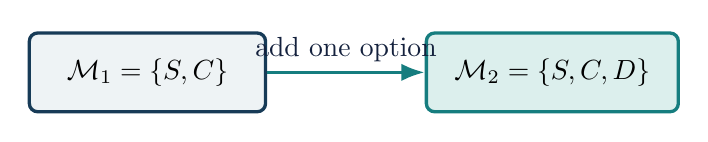
\begin{tikzpicture}[node distance=1.0cm,>=Latex]
      \node[draw=Navy,very thick,rounded corners=3pt,fill=Mist,minimum width=3.0cm,minimum height=1.0cm]
        (m1) {$\mathcal M_1=\{S,C\}$};
      \node[draw=Teal,very thick,rounded corners=3pt,fill=Mint,minimum width=3.2cm,minimum height=1.0cm,right=2.0cm of m1]
        (m2) {$\mathcal M_2=\{S,C,D\}$};
      \draw[->,very thick,Teal] (m1) -- node[above,Ink]{add one option} (m2);
    \end{tikzpicture}
  \end{center}

  \[
    \mathcal M_1\subset\mathcal M_2
    \quad\Longrightarrow\quad
    V^2_{ik,t}\ge V^1_{ik,t}
    \quad\Longrightarrow\quad
    Z^2_{ik,t}\ge Z^1_{ik,t}
    \quad\Longrightarrow\quad
    N^2_{it}\ge N^1_{it}.
  \]

  \begin{beamercolorbox}[wd=\textwidth,sep=0.18cm,rounded=true]{block body example}
    \textbf{Why only weak?} If delegation is unattractive, the developer ignores it. The result holds \textbf{path by path}, without a distributional assumption.
  \end{beamercolorbox}

  \vspace{0.20cm}
  \centering\small
  Strict expansion at date $t$ additionally needs some language with
  $V^1_{ik,t}<0\le V^D_{ik,t}$.
\end{frame}

% -------------------------------------------------------------------
\begin{frame}{6. Proposition 2: the delegation advantage creates an activation band}
  \vspace{-0.10cm}
  \[
    \boxed{
    B\equiv T^S-T^D
    =\lambda\bigl[az(A)-s\mu\bigr]-\kappa(a,s)-r_D
    +\frac{\rho}{2}
      \left[
        \frac{(2\lambda-\lambda^2)s^2}{\pi}
        -\sigma_D^2(a,s,A)
      \right]}
  \]

  \vspace{-0.06cm}
  \begin{center}
    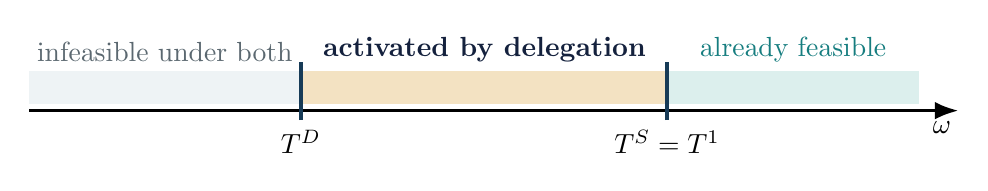
\begin{tikzpicture}[x=1cm,y=1cm]
      \draw[very thick,-{Latex[length=3mm]}] (0,0) -- (11.8,0);
      \fill[Mist] (0,0.08) rectangle (3.45,0.50);
      \fill[Gold!32] (3.45,0.08) rectangle (8.10,0.50);
      \fill[Mint] (8.10,0.08) rectangle (11.30,0.50);
      \draw[very thick,Navy] (3.45,-0.12) -- (3.45,0.62);
      \draw[very thick,Navy] (8.10,-0.12) -- (8.10,0.62);
      \node[below] at (3.45,-0.12) {$T^D$};
      \node[below] at (8.10,-0.12) {$T^S=T^1$};
      \node[above,Slate] at (1.72,0.50) {infeasible under both};
      \node[above,Ink,font=\bfseries] at (5.78,0.50) {activated by delegation};
      \node[above,Teal] at (9.70,0.50) {already feasible};
      \node[below right] at (11.35,-0.02) {$\omega$};
    \end{tikzpicture}
  \end{center}

  \vspace{0.04cm}
  \[
    B>0
    \quad\Longrightarrow\quad
    Z^2_{ik,t}-Z^1_{ik,t}
      =\mathbf 1\!\left[T^D_{ik,t}\le\omega_{ik,t}<T^S_{ik,t}\right].
  \]

  \centering\scriptsize
  A positive-width band is not yet strict expected expansion: the opportunity distribution must put positive mass inside it.
\end{frame}

% -------------------------------------------------------------------
\begin{frame}{7. What I verified by hand}
  \begin{columns}[T,onlytextwidth]
    \begin{column}{0.61\textwidth}
      \source{Relabeled here into the paper's printed notation.}
      \vspace{-0.10cm}
      {\footnotesize\begin{align*}
        B
        &=T^S-T^D\\[0.06cm]
        &=\left[b-s\mu+\frac{\rho s^2}{2\pi}\right]
        -\left[
          b-(1-\lambda)s\mu-\lambda az(A)\right.\\[-0.05cm]
        &\hspace{1.5cm}\left.
          +\kappa(a,s)+r_D
          +\frac{\rho}{2}
          \left(\frac{(1-\lambda)^2s^2}{\pi}+\sigma_D^2\right)
        \right]\\[0.06cm]
        &=\lambda[az(A)-s\mu]-\kappa(a,s)-r_D
          +\frac{\rho}{2}
          \left[
            \frac{(2\lambda-\lambda^2)s^2}{\pi}-\sigma_D^2
          \right].
      \end{align*}}
    \end{column}
    \begin{column}{0.35\textwidth}
      \begin{exampleblock}{Hand checks}
        \small
        \begin{itemize}
          \item rearrange $V^D\ge0$ without flipping a sign;
          \item cancel the common activation cost $b$;
          \item use $1-(1-\lambda)^2=2\lambda-\lambda^2$;
          \item recover $B>0\Rightarrow T^D<T^S$ and the half-open band.
        \end{itemize}
      \end{exampleblock}
    \end{column}
  \end{columns}

  \vspace{0.06cm}
  \begin{alertblock}{Scope of this evidence}
    \small The handwritten PDF is a human algebra check. It is \textbf{not} itself machine-verified; Lean separately checks formal declarations encoded from the model.
  \end{alertblock}
\end{frame}

% -------------------------------------------------------------------
\begin{frame}[fragile]{8. Mandatory Lean link: Proposition 2, objects and conclusion}
  \vspace{-0.06cm}
  \textbf{Paper equation (8):}
  \[
    Z^2_{ik,t}-Z^1_{ik,t}
    =\mathbf 1\!\left[T^D_{ik,t}\le\omega_{ik,t}<T^S_{ik,t}\right],
    \qquad B_{ik,t}>0.
  \]

  \vspace{-0.14cm}
  \begin{columns}[T,onlytextwidth]
    \begin{column}{0.61\textwidth}
\begin{lstlisting}[basicstyle=\ttfamily\fontsize{7.2}{8.1}\selectfont]
theorem threshold_indicator_sub_eq_band
    {delegationThreshold soloThreshold opportunity : ℝ}
    (hthreshold : delegationThreshold < soloThreshold) :
    ((if delegationThreshold ≤ opportunity then 1 else 0) : ℤ) -
        (if soloThreshold ≤ opportunity then 1 else 0) =
      if delegationThreshold ≤ opportunity ∧ opportunity < soloThreshold then 1 else 0 := by
  by_cases hdelegation : delegationThreshold ≤ opportunity
  · by_cases hsolo : soloThreshold ≤ opportunity
\end{lstlisting}
      \source{Real contiguous fragment from \texttt{lean/MainTheorems.lean}.}
    \end{column}
    \begin{column}{0.35\textwidth}
      \begin{block}{Economic $\leftrightarrow$ Lean}
        \scriptsize
        \begin{tabular}{@{}ll@{}}
          $T^D$ & \texttt{delegationThreshold}\\
          $T^S=T^1$ & \texttt{soloThreshold}\\
          $\omega$ & \texttt{opportunity}\\
          \shortstack[l]{$B>0$ implies\\$T^D<T^S$} & \texttt{hthreshold}\\
          activation & two threshold indicators
        \end{tabular}
      \end{block}
      \begin{exampleblock}{Exactness statement}
        \scriptsize The fragment proves the exact pointwise band identity conditional on $T^D<T^S$. Assumption 1 supplies $T^1=T^S$ outside this theorem. The full Proposition-2 interface also proves the atomless-measure/CDF claim and is judged \textbf{Matches}.
      \end{exampleblock}
    \end{column}
  \end{columns}
\end{frame}

% -------------------------------------------------------------------
\begin{frame}[fragile]{9. Lean finding \#1: Proposition 3 is not strictly true on its printed domain}
  \vspace{-0.06cm}
  \textbf{Printed dynamic claim:}
  \[
    \Delta C_i(s)=\sum_{k\in\mathcal U_i}
      \left[(1-p^1_{ik})^{s+1}-(1-p^2_{ik})^{s+1}\right]\ge0,
  \]
  with strict increase and concavity in the closed-frontier benchmark $p^1_{ik}=0<p^2_{ik}$.

  \vspace{-0.15cm}
  \begin{columns}[T,onlytextwidth]
    \begin{column}{0.40\textwidth}
      \begin{alertblock}{Two missing conditions}
        \scriptsize
        \begin{itemize}
          \item If $\mathcal U_i=\varnothing$, the sum is identically zero.
          \item The printed domain allows $p^2=1$; then the gap reaches one immediately and is constant afterward.
        \end{itemize}
      \end{alertblock}
      \begin{exampleblock}{Corrected strict result}
        \scriptsize Lean proves strict growth and strict concavity when the frontier is nonempty and every relevant hazard satisfies
        \[
          0<p^2_{ik}<1.
        \]
        These are \textbf{additional conditions}, not printed assumptions.
      \end{exampleblock}
    \end{column}
    \begin{column}{0.56\textwidth}
\begin{lstlisting}[basicstyle=\ttfamily\fontsize{7.0}{7.8}\selectfont]
theorem closed_frontier_gap_strict_mono
    {Language : Type*} (unfamiliar : Finset Language) (hazard : Language → ℝ)
    (hne : unfamiliar.Nonempty)
    (hpos : ∀ language ∈ unfamiliar, 0 < hazard language)
    (hlt : ∀ language ∈ unfamiliar, hazard language < 1) (horizon : ℕ) :

theorem dynamic_strictness_boundary_counterexample :
    ¬ ((1 - (1 - (1 : ℝ)) ^ (0 + 1)) < (1 - (1 - (1 : ℝ)) ^ (0 + 2))) := by
  norm_num
\end{lstlisting}
      \source{Verbatim excerpts from \texttt{lean/MainTheorems.lean}; the first conclusion is omitted. \texttt{closed\_frontier\_gap\_strict\_concave} uses the same conditions.}
    \end{column}
  \end{columns}
\end{frame}

% -------------------------------------------------------------------
\begin{frame}[fragile]{10. Lean finding \#2: strict repository expansion needs opportunity mass}
  \vspace{-0.08cm}
  \begin{columns}[T,onlytextwidth]
    \begin{column}{0.43\textwidth}
      \begin{block}{What the paper displays}
        \scriptsize Lower entry costs imply weakly more expected repository access; it states strict expansion when some repositories require languages in the activation band.
      \end{block}

      \vspace{-0.10cm}
      {\small\[
        \begin{gathered}
          c_r(\ell(r),2)\le c_r(\ell(r),1)\\[-0.04cm]
          \Longrightarrow\quad \mathbb E[R_i^2]\ge\mathbb E[R_i^1].
        \end{gathered}
      \]}
      \vspace{-0.10cm}

      \begin{alertblock}{What strictness additionally needs}
        \scriptsize For at least one repository,
        \[
          \Pr\!\left(c_r^2\le\Omega_{ir,t}<c_r^1\right)>0.
        \]
        The source proof uses this premise; the displayed proposition omits it.
      \end{alertblock}
    \end{column}
    \begin{column}{0.53\textwidth}
      \textcolor{Navy}{\scriptsize\bfseries Declaration}
\begin{lstlisting}[basicstyle=\ttfamily\fontsize{8.0}{8.8}\selectfont]
theorem repository_expected_expansion_strict
\end{lstlisting}
      \vspace{0.05cm}
      \textcolor{Navy}{\scriptsize\bfseries Decisive assumption}
\begin{lstlisting}[basicstyle=\ttfamily\fontsize{7.4}{8.2}\selectfont]
    (hband : ∃ repository ∈ repositories,
      0 < (opportunityLaw repository).real
        (Set.Ico (newCost repository) (oldCost repository))) :
\end{lstlisting}
      \source{Two verbatim excerpts from the same declaration in \texttt{lean/MainTheorems.lean}; intervening parameters and the conclusion are omitted.}

      \begin{exampleblock}{Lean verdict}
        \scriptsize
        \texttt{repository\_expected\_expansion} proves the paper's weak claim as stated. The displayed fragment proves strict expansion only after adding positive mass in a lowered-cost interval.
      \end{exampleblock}
    \end{column}
  \end{columns}
\end{frame}

% -------------------------------------------------------------------
\begin{frame}{11. Empirical evidence: sharp associations at first detectable use}
  \vspace{-0.03cm}
  \begin{columns}[c,onlytextwidth]
    \begin{column}{0.30\textwidth}\centering
      \metric{+2.528}{active programming languages}{event time $t=0$}
    \end{column}
    \begin{column}{0.30\textwidth}\centering
      \metric{+1.193}{newly used languages}{event time $t=0$}
    \end{column}
    \begin{column}{0.30\textwidth}\centering
      \metric{+0.382}{Shannon language entropy}{event time $t=0$}
    \end{column}
  \end{columns}

  \vspace{0.18cm}
  \begin{columns}[T,onlytextwidth]
    \begin{column}{0.47\textwidth}
      \begin{block}{Design and measurement}
        \scriptsize
        \begin{itemize}
          \item 5,346 developers; 28 months; 57.2 million changed files.
          \item Adoption: first commit with the machine-readable \texttt{Co-Authored-By: Claude} trailer.
          \item Doubly robust staggered-adoption event study, not-yet-treated comparisons, one month of anticipation.
        \end{itemize}
      \end{block}
    \end{column}
    \begin{column}{0.47\textwidth}
      \begin{exampleblock}{Economic mapping}
        \scriptsize
        \begin{itemize}
          \item active languages $\rightarrow$ production-set expansion;
          \item newly used languages $\rightarrow$ activation-band analogue;
          \item entropy $\rightarrow$ nontrivial diversification.
        \end{itemize}
      \end{exampleblock}
    \end{column}
  \end{columns}

  \begin{alertblock}{Interpretation boundary}
    \scriptsize These are \textbf{event-time associations}, not definitive causal effects. Adoption may occur when an unfamiliar-language project shock arrives.
  \end{alertblock}
\end{frame}

% -------------------------------------------------------------------
\begin{frame}{12. Where I did not believe the AI}
  \vspace{-0.03cm}
  \begin{columns}[T,onlytextwidth]
    \begin{column}{0.48\textwidth}
      \begin{block}{1. Citation / hallucination test}
        \scriptsize The initial title, \emph{Coding Beyond Your Training}, was not fabricated: it was the genuine v1 title. I did not infer v2 authors, sample, or results until checking the source.
      \end{block}

      \begin{block}{2. Notation correction}
        \scriptsize The v2 paper prints $\omega$ (opportunity), $\pi$ (precision), $\rho$ (risk aversion), $\gamma$ (conversational gain), $\lambda$ (delegated share), and $\kappa(a,s)$ (verification cost). Repository summary/hand notes re-letter several of these; this deck follows the paper.
      \end{block}
    \end{column}
    \begin{column}{0.48\textwidth}
      \begin{alertblock}{3. ``$T^D$ does not require skill''}
        \scriptsize Not as mathematical independence. $T^D$ still depends on $s$ through retained human execution, $\kappa(a,s)$, remaining human-match risk, and $\sigma_D^2(a,s,A)$. The defensible claim is narrower: the principal delegated-output term $\lambda az(A)$ does not require a positive language-specific foothold.
      \end{alertblock}

      \begin{exampleblock}{4. Different margin from Aouad--Lykouris--Zhong}
        \scriptsize
        \textbf{Aouad--Lykouris--Zhong:} AI substitutes for human implementation input inside an already feasible task.\par\smallskip
        \textbf{Quispe--Xu:} delegation can relax an entry/participation constraint and change which language--task opportunities are feasible.
      \end{exampleblock}
    \end{column}
  \end{columns}
\end{frame}

% -------------------------------------------------------------------
\begin{frame}{13. Final takeaway: frontier expansion, with conditions}
  \begin{beamercolorbox}[wd=\textwidth,sep=0.16cm,rounded=true]{block body example}
    \centering
    {\normalsize\bfseries Agentic AI can expand a developer's feasible production frontier by lowering the entry threshold for unfamiliar-language opportunities.}\par
    \smallskip
    It need not expand unaided human skill, and it need not activate opportunities with no probability mass in the lowered-threshold region.
  \end{beamercolorbox}

  \vspace{0.14cm}
  {\small\begin{tabular}{@{}p{0.22\textwidth}p{0.70\textwidth}@{}}
    \toprule
    \textbf{Claim} & \textbf{Formal-verification takeaway}\\
    \midrule
    Proposition 1 & Weak pathwise frontier expansion follows exactly from menu inclusion.\\
    Proposition 2 & The activation-band identity and nonnegative expected expansion are proved as stated.\\
    Proposition 3 & Strict dynamics require $\mathcal U_i\ne\varnothing$ and $0<p^2_{ik}<1$; the printed strict clause is false at allowed boundaries.\\
    Proposition 5 & Weak repository expansion is valid; strict expansion requires positive opportunity mass in a lowered-cost interval.\\
    \bottomrule
  \end{tabular}}

  \vspace{0.02cm}
  \begin{alertblock}{EconCSLib closeout status}
    \scriptsize \textbf{Partially formalized}; human review \textbf{0/9}. \textbf{Fast check passed}; no \texttt{sorry}/\texttt{admit}. Passing the encoded proofs does \textbf{not} establish semantic equivalence to every paper claim.
  \end{alertblock}
\end{frame}

\end{document}
